\documentclass{article}
\usepackage{graphicx} % Required for inserting images
\usepackage[section]{placeins}
\usepackage{float}

\title{Assignment 2}
\date{November 10, 2023}
\author{
  Ravi Raghavan\\
  \texttt{rr1133}
  \and
  Michelle Han\\
  \texttt{mmh255}
}
\begin{document}

%%%%%%%%% PART 1 %%%%%%%%%%%%%%%%%%%
\maketitle
\section{Motion Planning for a 2-link Planar Arm}
% SECTION 1.1
\subsection{Sampling Random Collision-Free Configurations}
% SECTION 1.1 FIGURES
\begin{figure}[h!]
     \begin{minipage}{0.48\textwidth}
    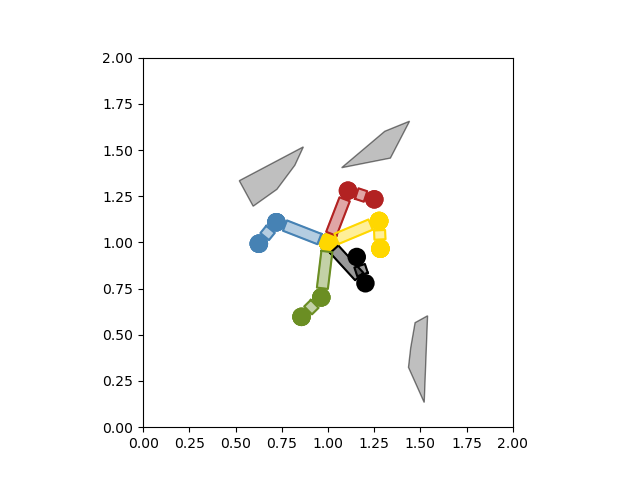
\includegraphics[width=\linewidth]{p1.1.1.png}
    \caption{Provided environment}
  \end{minipage}\hfill
  \begin{minipage}{0.48\textwidth}
    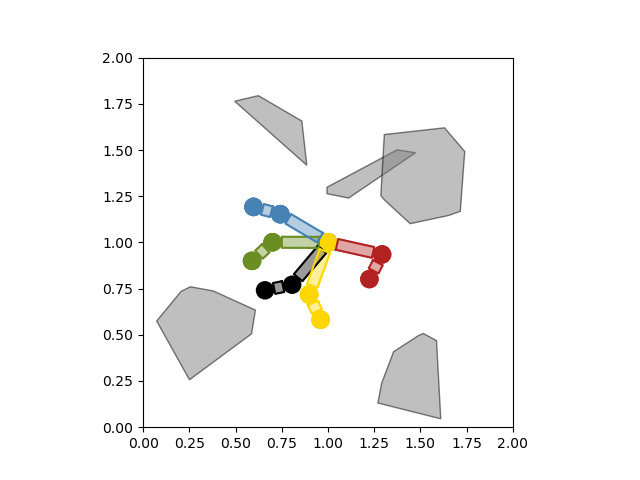
\includegraphics[width=\linewidth]{p1.1.2.png}
    \caption{Assignment 1 environment}
  \end{minipage}\hfill
\end{figure}
% SECTION 1.2
\subsection{Nearest Neighbors}
To find the nearest neighbors, the distance was measured using the end-effector positions. For implementation, forward kinematics was used to determine the coordinates of the end-effectors and the Eucliean distance was calculated from the coordinates.
% SECTION 1.2 FIGURES
\begin{figure}[htbp]
  \centering
  \begin{minipage}{0.45\textwidth}
    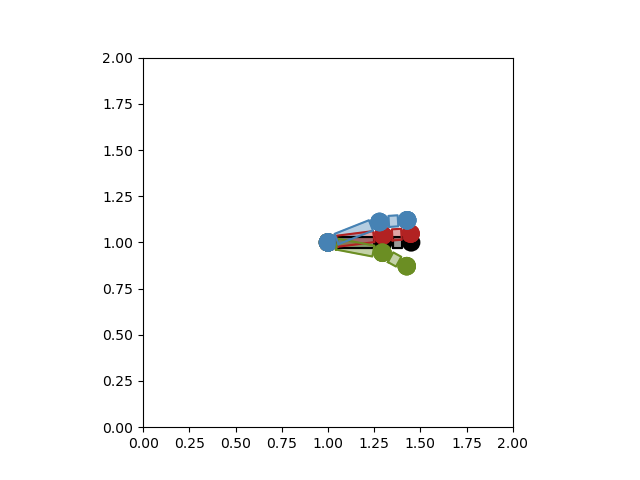
\includegraphics[width=\linewidth]{p1.2.1.png}
    \caption{target = [0,0], k=3}
  \end{minipage}\hfill
  \begin{minipage}{0.45\textwidth}
    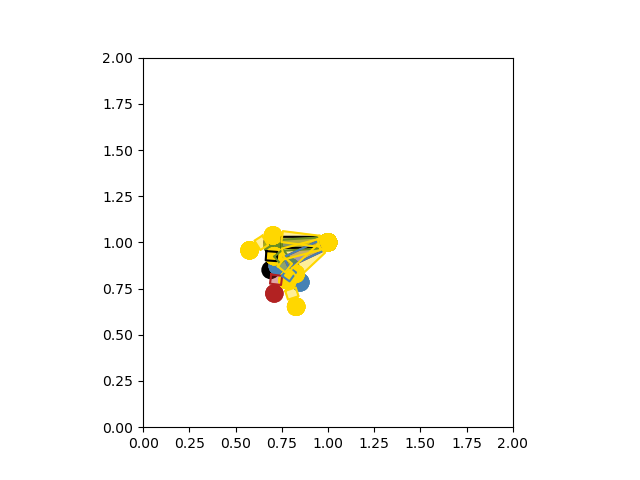
\includegraphics[width=\linewidth]{p1.2.2.png}
    \caption{target = [3.14,1.5], k=6}
  \end{minipage}
  \begin{minipage}{0.45\textwidth}
    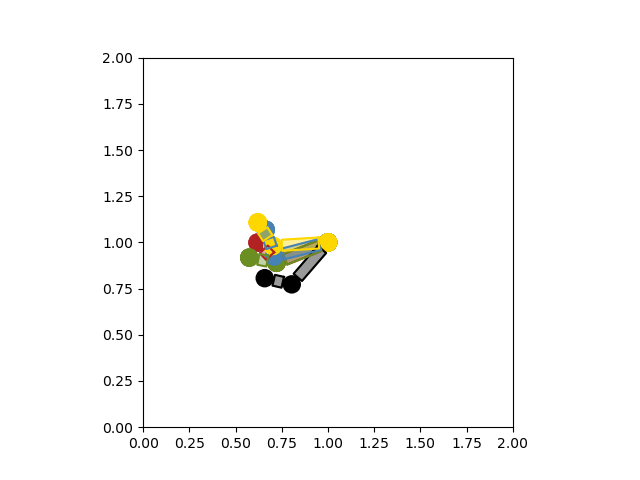
\includegraphics[width=\linewidth]{p1.2.3.png}
    \caption{target = [4,5.2], k=4}
  \end{minipage}\hfill
  \begin{minipage}{0.45\textwidth}
    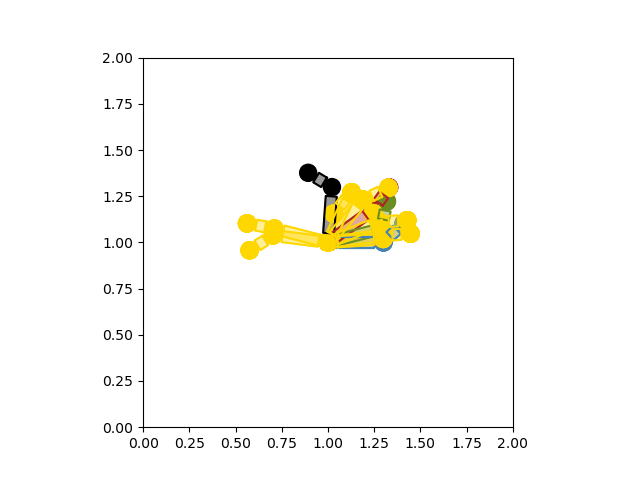
\includegraphics[width=\linewidth]{p1.2.4.png}
    \caption{target = [1.5,1.1], k=10}
  \end{minipage}
   \begin{minipage}{0.45\textwidth}
    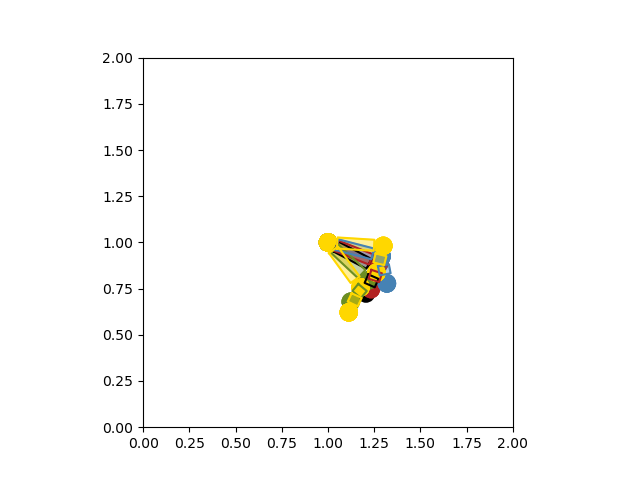
\includegraphics[width=\linewidth]{p1.2.5.png}
    \caption{target = [5.8,-1.5], k=5}
  \end{minipage}
\end{figure}
\subsubsection{With Linear Search Approach}
To implement the Linear Search,
% SECTION 1.2 -> EXTRA CREDIT
\subsubsection{With KD-Tree Search Approach}
To implement the KD-Tree Search,
\subsubsection{Search Comparison}
To compare running times between linear search and kd-tree search, the map used was arm\_polygons.npy and the target was [3.14, 0]. When comparing the running time as the number of configurations increased, the k nearest neighbors was set to 3. When comparing the running time as the number of neighbors increased, the number of random configurations was 100. 
\begin{figure}[]
  \centering
    \includegraphics[width=\linewidth]{comp_k.png}
    \caption{Running time vs. number of nearest neighbors}
    \includegraphics[width=\linewidth]{comp_configs.png}
    \caption{Running time vs. number of configurations}
\end{figure}
\subsubsection{Visualizations}
\begin{figure}[htbp]
  \centering
  \begin{minipage}{0.45\textwidth}
    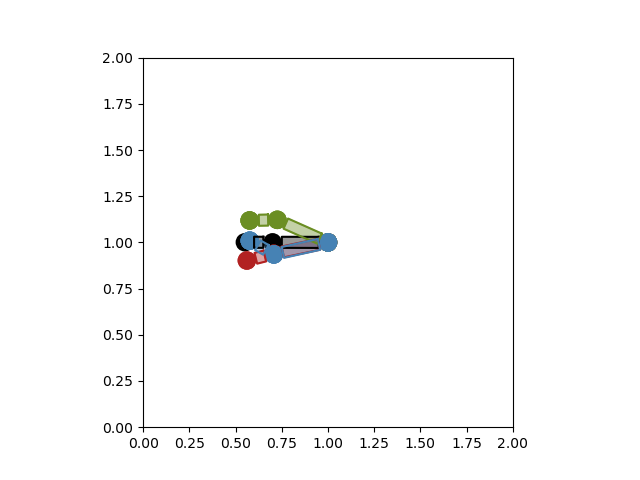
\includegraphics[width=\linewidth]{p1.2.ec100.png}
    \caption{}
  \end{minipage}\hfill
  \begin{minipage}{0.45\textwidth}
    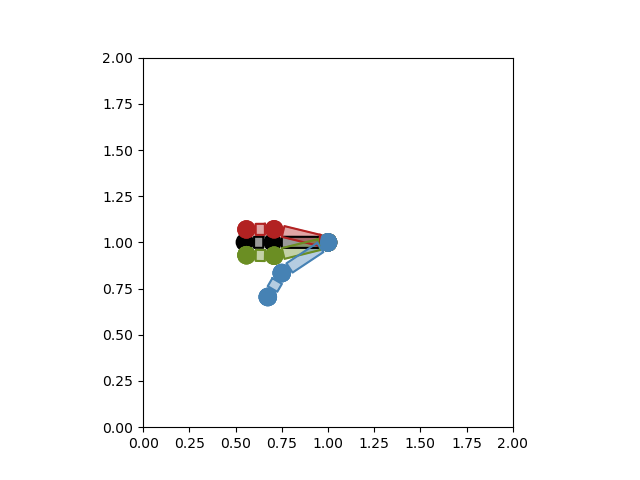
\includegraphics[width=\linewidth]{p1.2.ec500.png}
    \caption{}
  \end{minipage}
  \begin{minipage}{0.45\textwidth}
    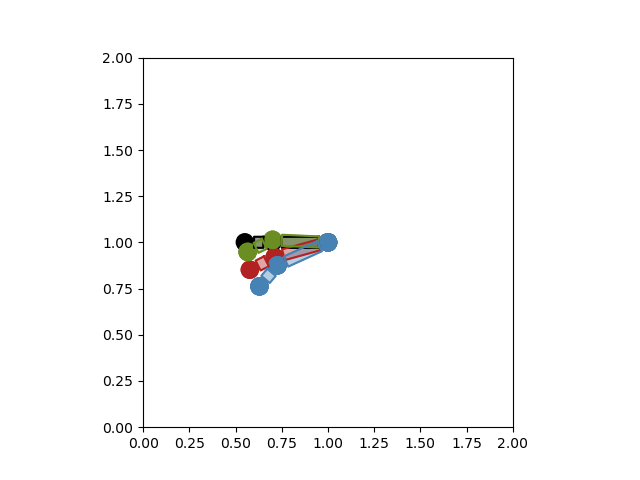
\includegraphics[width=\linewidth]{p1.2.ec1000.png}
    \caption{}
  \end{minipage}\hfill
  \begin{minipage}{0.45\textwidth}
    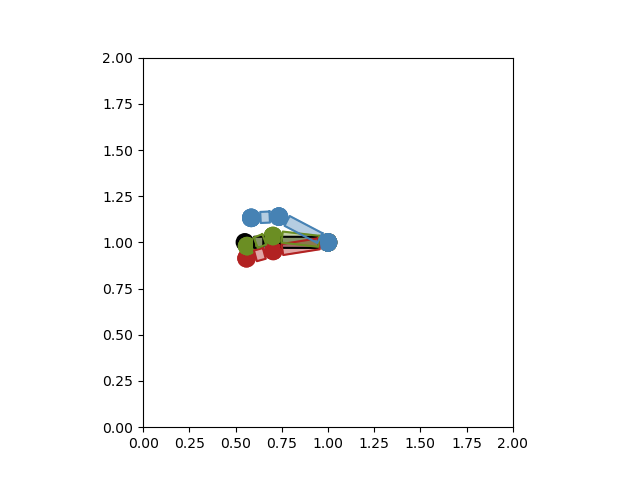
\includegraphics[width=\linewidth]{p1.2.ec2000.png}
    \caption{}
  \end{minipage}
\end{figure}
\begin{figure}[htbp]
  \centering
  \begin{minipage}{0.45\textwidth}
    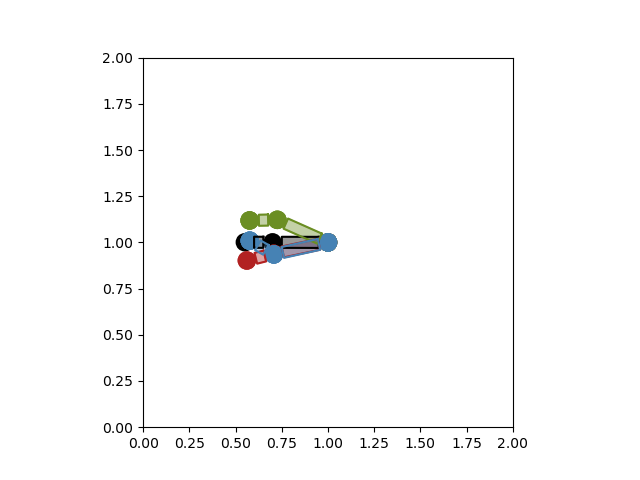
\includegraphics[width=\linewidth]{p1.2.ec3n.png}
    \caption{}
  \end{minipage}\hfill
  \begin{minipage}{0.45\textwidth}
    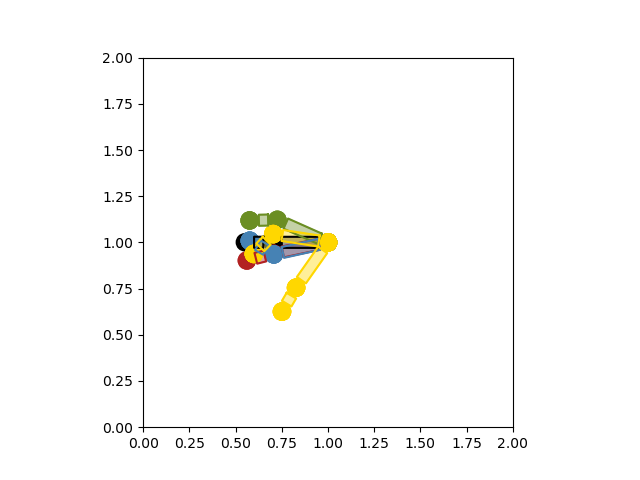
\includegraphics[width=\linewidth]{p1.2.ec5n.png}
    \caption{}
  \end{minipage}
  \begin{minipage}{0.45\textwidth}
    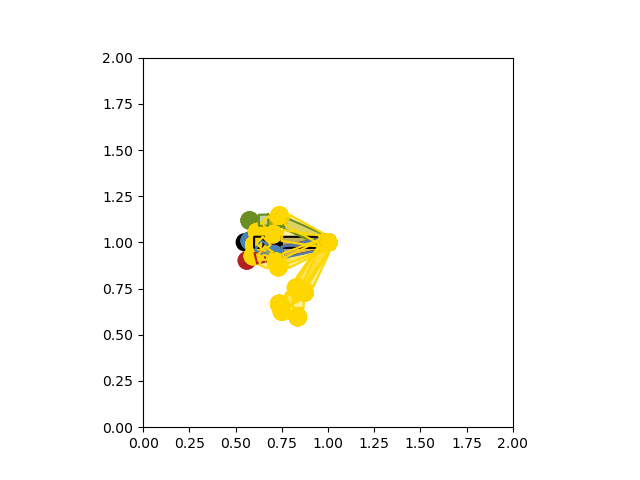
\includegraphics[width=\linewidth]{p1.2.ec10n.png}
    \caption{}
  \end{minipage}\hfill
  \begin{minipage}{0.45\textwidth}
    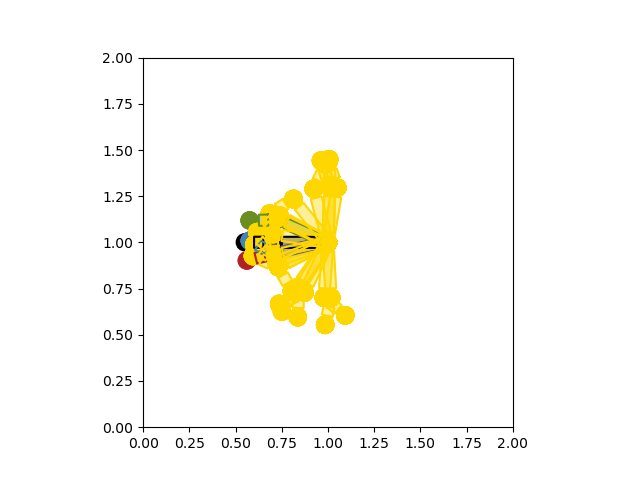
\includegraphics[width=\linewidth]{p1.2.ec20n.png}
    \caption{}
  \end{minipage}
\end{figure}
% SECTION 1.3
\subsection{Interpolation Along the Straight Line in the C-Space}
describe implementation and resulting visualizations
% SECTION 1.4
\subsection{RRT Implementation}
explain RRT implementation
how did i decide to add an edge to tree
% SECTION 1.5
\subsection{PRM Implementation}
explain PRM implementation
% SECTION 1.6 -> EXTRA CREDIT
\subsubsection{PRM*}
explain PRMstar and how i changed PRM
\subsubsection{Planner Comparison}
%%%%%%%%% PART 2 %%%%%%%%%%%%%%%%%%%
\maketitle
\section{Motion Planning for a Rigid Body in 2D}
% SECTION 2.1
\subsection{Sampling Random Collision-Free Configurations}
% SECTION 2.2
\subsection{Nearest Neighbors with Linear Search Approach}
% SECTION 2.3
\subsection{Interpolation Along the Straight Line in the C-Space}
% SECTION 2.4
\subsection{RRT Implementation}
% SECTION 2.5
\subsection{PRM Implementation}
%%%%%%%%% PART 3 %%%%%%%%%%%%%%%%%%%
\maketitle
\section{Motion Planning for a First-Order Car}
% SECTION 3.1
\subsection{Implementation of Dynamics}
% SECTION 3.2
\subsection{Integration of Dynamics}
% SECTION 3.3
\subsection{RTT and Planning with Dynamics}

\end{document}
